\section{Mergeable Data Type}

\begin{figure}[!t]
\centering
\subcaptionbox[] {\small
  When a thread \C{pushes} a new version, it is presumably a semantic
  successor of the version it last \C{pulled} into the heap.
  \label{fig:syntactic-ancestor-1}
} [0.47\columnwidth] {
  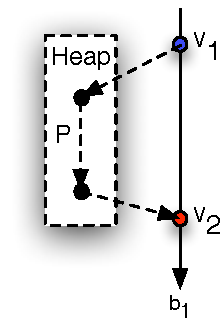
\includegraphics[scale=0.7]{Figures/semantic-ancestor-1}
}
\hfill
\subcaptionbox[] {\small
  Versions created by the \C{merge} operation are syntactic successors
  of merged versions, but need not necessarily be semantic successors.
  \label{fig:syntactic-ancestor-2}
} [0.47\columnwidth] {
  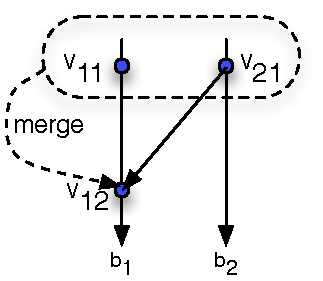
\includegraphics[scale=0.8]{Figures/semantic-ancestor-2}
}
\caption{New versions are created from existing versions either
through \C{push} or \C{merge}.}
\label{fig:syntactic-ancestors}
\end{figure}

\begin{figure}
\centering
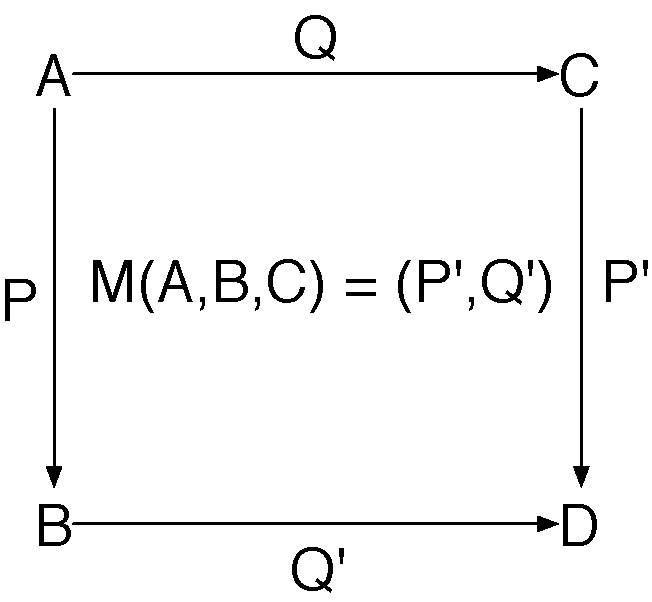
\includegraphics[scale=0.4]{Figures/pushouts}

\caption{Commutative diagram representing the merge operation.}
\label{fig:pushouts}
\end{figure}

We now formally define what we mean by a mergeable type. The
definition serves as a guide to write merge functions for functional
data types, and elevate them to the level of replicated data types.

A functional data type library is as a tuple consisting of a type
($t$), and a (possibly infinite) collection of functions ($f$, $g$,
etc.) of type $t \rightarrow t$. We call the functions \emph{primitive
morphisms}\footnote{We borrow terminology from category theory for
convenience}. A morphism ($P$, $Q$, etc.) is either a primitive
morphism, or an associative composition of morphisms ($P \circ Q \circ
R$). An object $B:t$ is called a \emph{semantic successor} of $A:t$
(conversely, $A$ is called a \emph{semantic ancestor} of $B$) if and
only if there exists a morphism $P$ such that $P(A) = B$.  

The aim of a three-way merge function over a type $t$ is to merge a
pair of semantic successors, $B:t$ and $C:t$, of an object $A:t$, into
another object $D:t$ such that the relationship between the semantic
successors and $D$ satisfies certain conditions. These conditions can
be understood by observing the \rulelabel{E-Pull-Wait} rule of of
Fig.~\ref{fig:opsem}, which applies the \C{merge} function to a pair
of concurrent versions ($v_1$ and $v_2$) and their least common
ancestor ($v$). Thus, the only relationship that exists between $v$
and $v_1$, and $v$ and $v_2$ is the syntactic ancestor relationship
that follows from the branching structure. The merge function, as
described above, however assumes that the concurrent versions are
semantic successors of their LCA. It is therefore essential to
maintain coherence between the syntactic and semantic ancestor
relations.

The ways in which syntactic ancestor relationships are created among
versions is captured in Fig.~\ref{fig:syntactic-ancestors}. Whenever an
object is pushed onto the branch, an ancestor relationship is created
between the previous version $v_1$, and the newly created version
$v_2$ (Fig.~\ref{fig:syntactic-ancestor-1}). However, since $v_2$ is
pushed by the thread after reading $v_1$ into the heap, it is
reasonable to assume that $v_2$ is a result of applying a morphism $P$
to $v_1$ (i.e., $\exists P.~v_2 = P(v_1)$).  Hence, $v_1$ is a
semantic ancestor of $v_2$.  Fig.~\ref{fig:syntactic-ancestor-2}
captures another way of establishing ancestor relationship, namely by
merging branches. Version $v_{21}$ on branch $b_2$ is merged into
$v_{11}$ on $b_1$ to create $v_{12}$ on $b_1$. Versions $v_{11}$ and
$v_{21}$ are now syntactic ancestors of $v_{12}$, but for them to be
semantic ancestors, merge function has to enforce the relationship
explicitly. In other words, the result of merging of a pair of
semantic successors, $B$ and $C$, of an $A$, has to be an object $D$
that is a semantic successor of both $B$ and $C$. We now formalize
this intuition to define a mergeable type.
\begin{definition} [\bfseries Mergeable Type]
A type $t$ is said to be mergeable, if and only if there exists a
function $M$ of type $t \times t \times t \rightarrow (t \rightarrow
t)\times(t \rightarrow t)$ that satisfies the following property:
$\forall (A, B, C\,:\,t).~ (\exists (P,Q\,:\, t \rightarrow t).~ B =
P(A) \conj C = Q(A)) \Rightarrow (\exists (P',Q': t\rightarrow
t).~M(A,B,C) = (P',Q') \conj  Q'(B) = P'(C))$
\end{definition}
Intuitively, a type $t$ is a mergeable type if, whenever there exist
two morphisms $P$ and $Q$ that map $A:t$ to $B:t$ and $C:t$, there
must also exist morphisms $P'$ and $Q'$, the map both $B$ and $C$ to
$D:t$. This intuition is expressed visusally in
Fig.~\ref{fig:pushouts}.

The three-way merge function \C{merge} can be defined
straightforwardly in terms of the function $M$ described above. Thus,
for a mergeable type $t$, we have the guarantee that a sequence of
values read by a thread from its branch ``makes sense'' as per the
data type semantics: 

\begin{theorem} [\bfseries Branch-local consistency]
Let $t$ be a mergeable type, and let $H$ be a legal branching history
over values of type $t$. For every pair of values $v_1:t$ and $v_2:t$
along a branch $b$ in $H$, if $\under{H}{v_1 \preceq v_2}$, then there
exists a morphism $P:t\rightarrow t$ such that $v_2 = P(v_1)$.
\end{theorem}

